\section{Link-State Database}
\label{sec:lsdb}

The Link-State Database (LSDB) holds LSA information distributed by other routers in the network.
The LSDB stores all three types of LSAs and will trigger necessary events when a new LSA is added, when an LSA is updated, and when an LSA expires.
The LSDB also handles LSA retrieval and validation, performs LSA builds, and triggers routing table calculations.

\subsection{Retrieving an LSA}

The LSDB provides \texttt{Lsdb::expressInterest()} as a public interface to retrieve an LSA from the network.
If LSA Data is returned, the LSDB will handle the Data validation and perform the necessary LSDB modifications.
If the LSA Interest times out, the LSDB will continue to re-attempt to fetch the LSA Data.
The LSDB will stop trying these fetch re-attempts once it has tried for as long as the maximum configurable LSA refresh time.

\subsection{Building LSAs}

The LSDB provides three interfaces to build and install a router's own various LSAs.
\begin{itemize}
\item \texttt{Lsdb::scheduleAdjLsaBuild()} schedules an Adjacency LSA calculation if one is not already scheduled and if hyperbolic routing is not turned on, i.e. if link-state routing or dry run is on.
\item \texttt{Lsdb::buildAndInstallOwnAdjLsa()} instantiates a new Adjacency LSA with the router's current adjacency list, incremented sequence number, and number of active neighbors. It also notifies the Sync Logic Handler to publish the routing update(Section~\ref{sssec:routing-update}) if link-state routing or dry-run is enabled to let other node in the network know the newly instlled Adjacency LSA.
\item \texttt{Lsdb::buildAndInstallOwnCoordinateLsa()} instantiates a new Coordinate LSA with the router's hyperbolic coordinates and an incremented sequence number. The newly constructed Coordinate LSA is then installed in the LSDB. It also notifies the Sync Logic Handler to publish the routing update(Section~\ref{sssec:routing-update}) if hyperbolic routing or dry run is turned on to let other nodes in the network know the newly installed Coordinate LSA.
\item \texttt{Lsdb::buildAndInstallOwnNameLsa()} instantiates a new Name LSA with the router's current name prefix list and an incremented sequence number. The newly constructed Name LSA is then installed in the LSDB.
\end{itemize}

\subsection{LSA Installation and Updates}

The LSDB provides three internal interfaces for each of the three types of LSAs to add or update LSAs in the LSDB.
The general logic for each type of LSA installation is similar (Figure~\ref{fig:generic-lsdb-flow}), but there are slight differences in the events that are triggered by an installation or update.

\begin{figure}[h]
\center
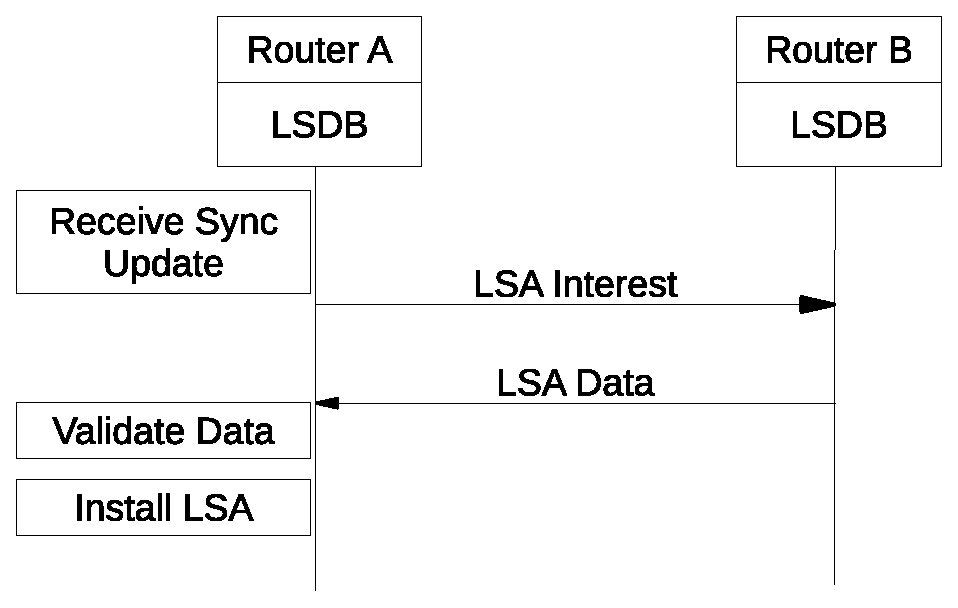
\includegraphics[width=0.5\linewidth]{figures/generic-lsdb-flow}
\label{fig:generic-lsdb-flow}
\caption{The general LSDB logic for each LSA type}
\end{figure}

\subsubsection{Lsdb::installAdjLsa()}

When an Adjacency LSA is passed to \texttt{Lsdb::installAdjLsa()}, the LSDB first attempts to find the LSA in its current database.

If the Adjacency LSA is not installed in the database, the LSA will first be added to the database.
If the installed LSA is advertised by a remote router, the remote router's name will be added to the NPT and the LSA will be scheduled to expire after the expiration time point included in the LSA.
Since a new Adjacency LSA introduces a new node and new links in the network, a routing table calculation is scheduled.

If the Adjacency LSA is already installed in the database, the existing LSA will only be updated if the newly received LSA has a higher sequence number.
If an Adjacency LSA with a higher sequence number is being installed, the existing LSA's sequence number and expiration time will be updated.
If the newly received LSA contains an adjacency list that is different from the existing LSA, the existing LSA's adjacencies are updated and a routing table calculation is scheduled to account for the network change.
Finally, if the updated LSA is advertised by a remote router, the LSA will be scheduled to expire after the expiration time point included in the LSA.

\subsubsection{Lsdb::installCoordinateLsa()}

When a Coordinate LSA is passed to \texttt{Lsdb::installCoordinateLsa()}, the LSDB first attempts to find the LSA in its current database.

If the Coordinate LSA is not installed in the database, the LSA will first be added to the database.
If the installed LSA is advertised by a remote router, the remote router's name will be added to the NPT, and the LSA will be scheduled to expire after the expiration time point included in the LSA.
If hyperbolic routing is enabled, a new Coordinate LSA means that the routing table should be re-calculated to include the new destination router.

If the Coordinate LSA is already installed in the database, the existing LSA will only be updated if the newly received LSA has a higher sequence number.
If a Coordinate LSA with a higher sequence number is being installed, the existing LSA's sequence number and expiration time will be updated.
If the newly received LSA contains hyperbolic coordinate different from the existing LSA, the existing LSA's coordinates are updated.
If hyperbolic routing is enabled, an LSA with new coordinates means the routing table should be re-calculated to account for the different coordinates.
Finally, If the updated LSA is advertised by a remote router, the LSA will be scheduled to expire after the expiration time point included in the LSA.

\subsubsection{Lsdb::installNameLsa()}

When a Name LSA is passed to \texttt{Lsdb::installNameLsa()}, the LSDB first attempts to find the LSA in its current database.

If the Name LSA is not installed in the database, the LSA will first be added to the database.
If the installed LSA is advertised by a remote router, the remote router's name and each advertised name in the LSA will be added to the NPT,  and the LSA will be scheduled to expire after the expiration time point included in the LSA.

If the Name LSA is already installed in the database, the existing LSA will only be updated if the newly received LSA has a higher sequence number.
If a Name LSA with a higher sequence number is being installed, the existing LSA's sequence number and expiration time will be updated.
A set difference is performed between the new LSA's advertised name prefix list and the existing LSA's advertised name prefix list to determine name prefixes that have been added.
If there are added name prefixes, the name prefixes are added to the NPT and to the existing LSA.
A set difference is then performed between the new LSA's advertised name prefix list and the existing LSA's advertised name prefix list to determine name prefixes that have been removed.
If there are removed name prefixes, the name prefixes are removed from the NPT and from the existing LSA.
Finally, If the updated LSA is advertised by a remote router, the LSA will be scheduled to expire after the expiration time point included in the LSA.

\subsection{LSA Expiration}

LSAs are scheduled to expire after a configurable amount of time in order to allow for LSDB cleanup when a router crashes.
After the expiration period, if the LSA belongs to the current router, the LSA is refreshed with an incremented sequence number (Section~\ref{sec:lsa-refresh}).
Otherwise, if the LSA belongs to a remote router, the LSA is removed from the LSDB.
Removing an LSA from the LSDB triggers different events depending on the type of the LSA.
\begin{itemize}
\item \textbf{Adjacency LSA} - When an Adjacency LSA is removed, a routing table calculation is scheduled to determine new paths that don't include the associated router.
\item \textbf{Coordinate LSA} - When a Coordinate LSA is removed and hyperbolic routing is enabled, a routing table calculation is scheduled.
\item \textbf{Name LSA} - When a Name LSA is removed, the name prefixes advertised by the LSA are removed from the NPT.
\end{itemize}

In all three cases, the LSA's origin router's name will also be removed from the NPT.

\subsection{LSA Refresh}
\label{sec:lsa-refresh}

When a router refreshes its own LSA, all three LSA types trigger the same events:
\begin{itemize}
\item Increment the LSA's sequence number by one
\item Schedule the LSA to expire after the configured \texttt{lsa-refresh-time}.
\item Publish a routing update in NSync to notify other routers of the change in the LSDB.
\end{itemize}


